\documentclass[12pt]{article}

\usepackage[spanish]{babel}
\usepackage[utf8]{inputenc}
\usepackage{graphicx}
\usepackage{geometry}
\usepackage{xcolor}
\usepackage{fancyhdr}
\usepackage{lastpage}
\usepackage{pdfpages}
\usepackage{listings}
\usepackage{schemata}

\geometry{top=25mm,left=15mm,right=15mm,a4paper}

\pagestyle{fancy}
\fancyhf{}
\lhead{Computación Concurrente}
\cfoot{Página \thepage\ de \pageref{LastPage}}

\graphicspath{./}

\begin{document}
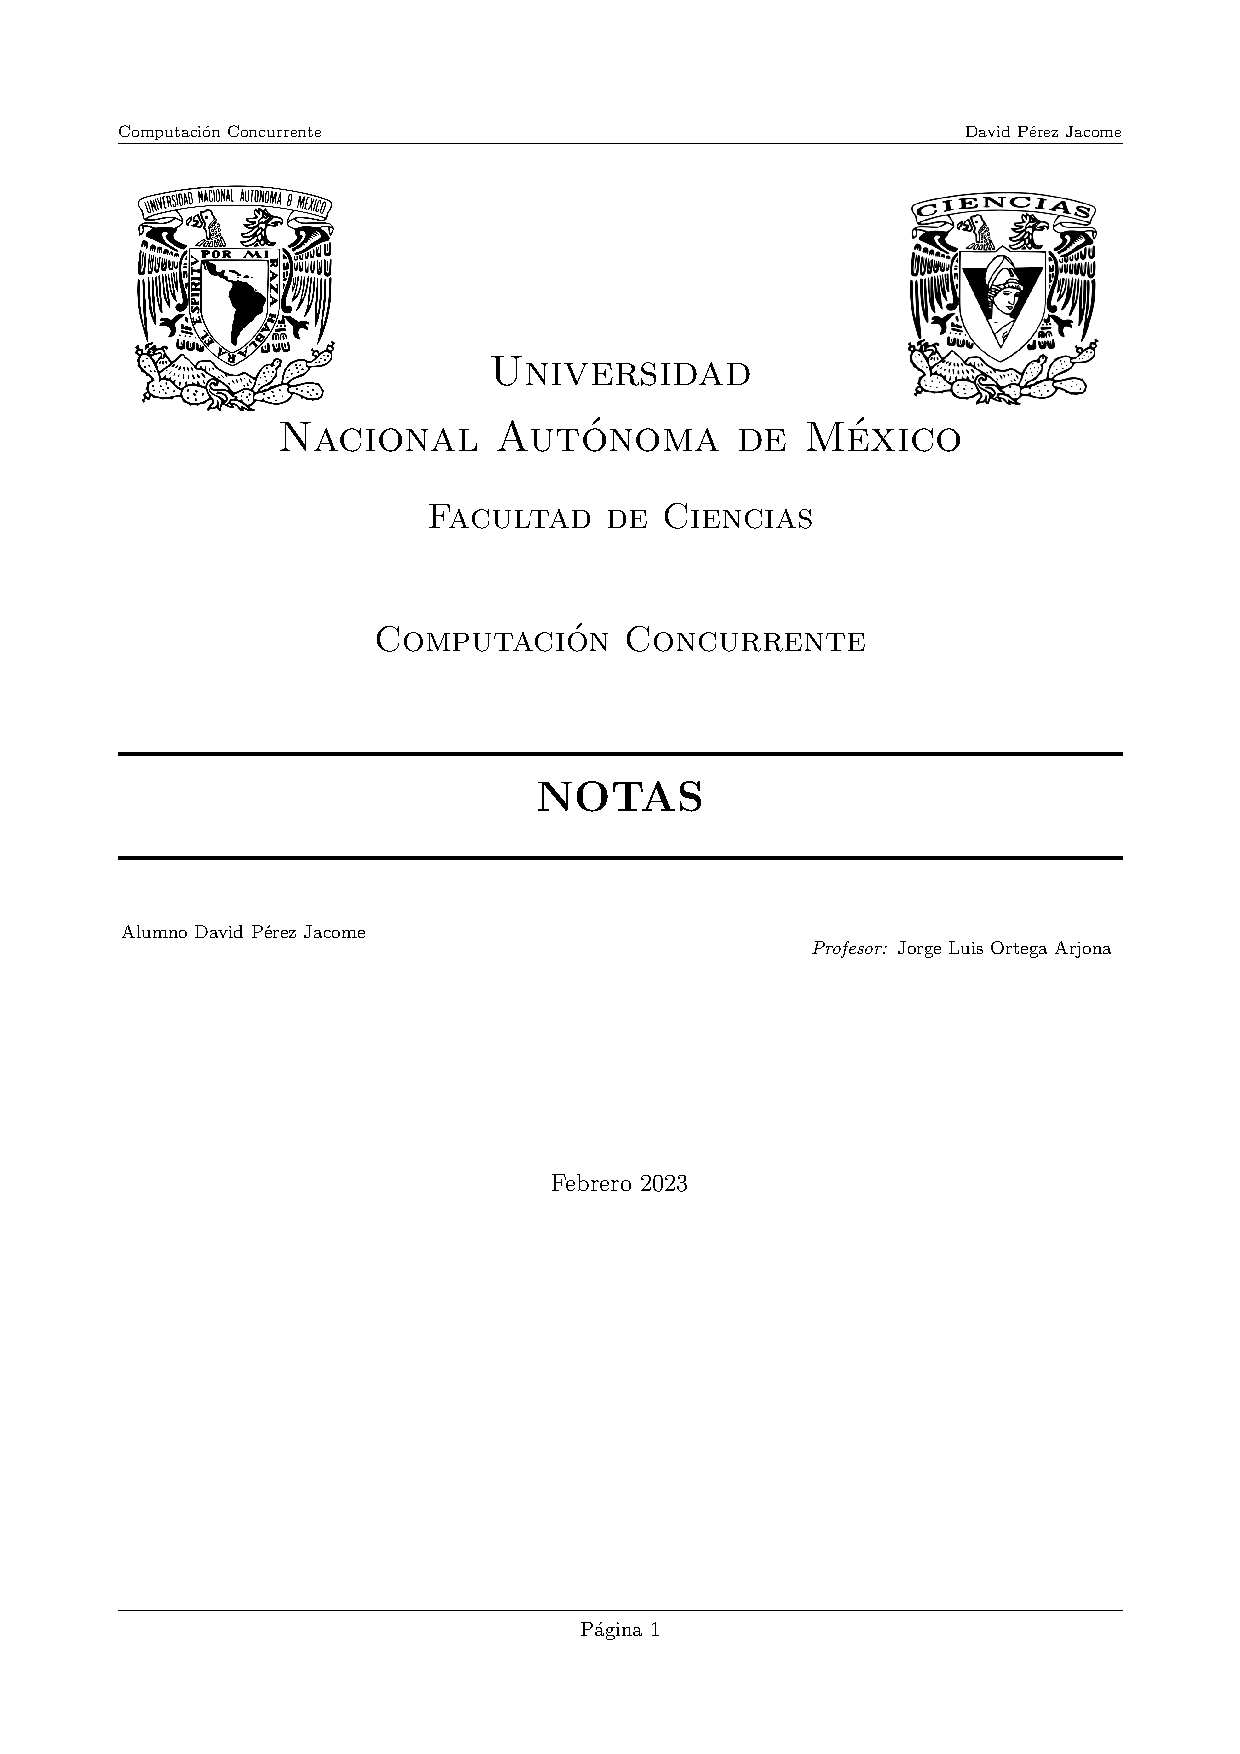
\includepdf{Portada.pdf}
{\color{blue} \section*{\textbf{Notas}}}
\vspace{1em}

{\color{blue} \subsection*{\textbf{TEMA 1: INTRODUCCIÓN.}}}

\subsubsection*{\textbf{Factores}}
\begin{enumerate}
    \item \textbf{1 Procesador}
    \begin{enumerate}
        \item tienen multithreading.
        \item memoria compartida.
    \end{enumerate}
    \item \textbf{N Procesadores} 
    \begin{enumerate}
        \item \textbf{Paralelo}(multiprocesadores o multicore).
        \begin{enumerate}
            \item \textbf{Memoria compartida}
            \begin{enumerate}
                \item Semaforos
                \item Región Critica
                \item Monitores
                \item Paso de mensajes
                \item Llamada a Proc. Remoto (RPC)
            \end{enumerate}
            \item \textbf{Memoria Distribuida}
        \end{enumerate}
        \item \textbf{Distribuido}(red de computadoras) 
    \end{enumerate}
    \item \textbf{Lenguajes de Programación}
    \item \textbf{Hardware}
\end{enumerate}
\vspace{-0.5em}
\subsubsection*{\textbf{PROGRAMACIÓN SECUENCIAL VS PROGRAMACIÓN CONCURRENTE}}
\begin{tabular}{| c | c |}
    \hline
    Secuencial & Concurrente \\ \hline
    Programa haga lo que deba hacer & Controlar el NO-Determinismo \\
    Programa que se detenga & Sincronizar procesos.
\end{tabular}
\\
\vspace{1em}

{\color{blue} \subsection*{\textbf{Factores de desempeño.}}}
\begin{enumerate}
    \item Plataforma de Hardware
    \item Lenguaje de Programación
    \item Problema de Resolución
\end{enumerate}

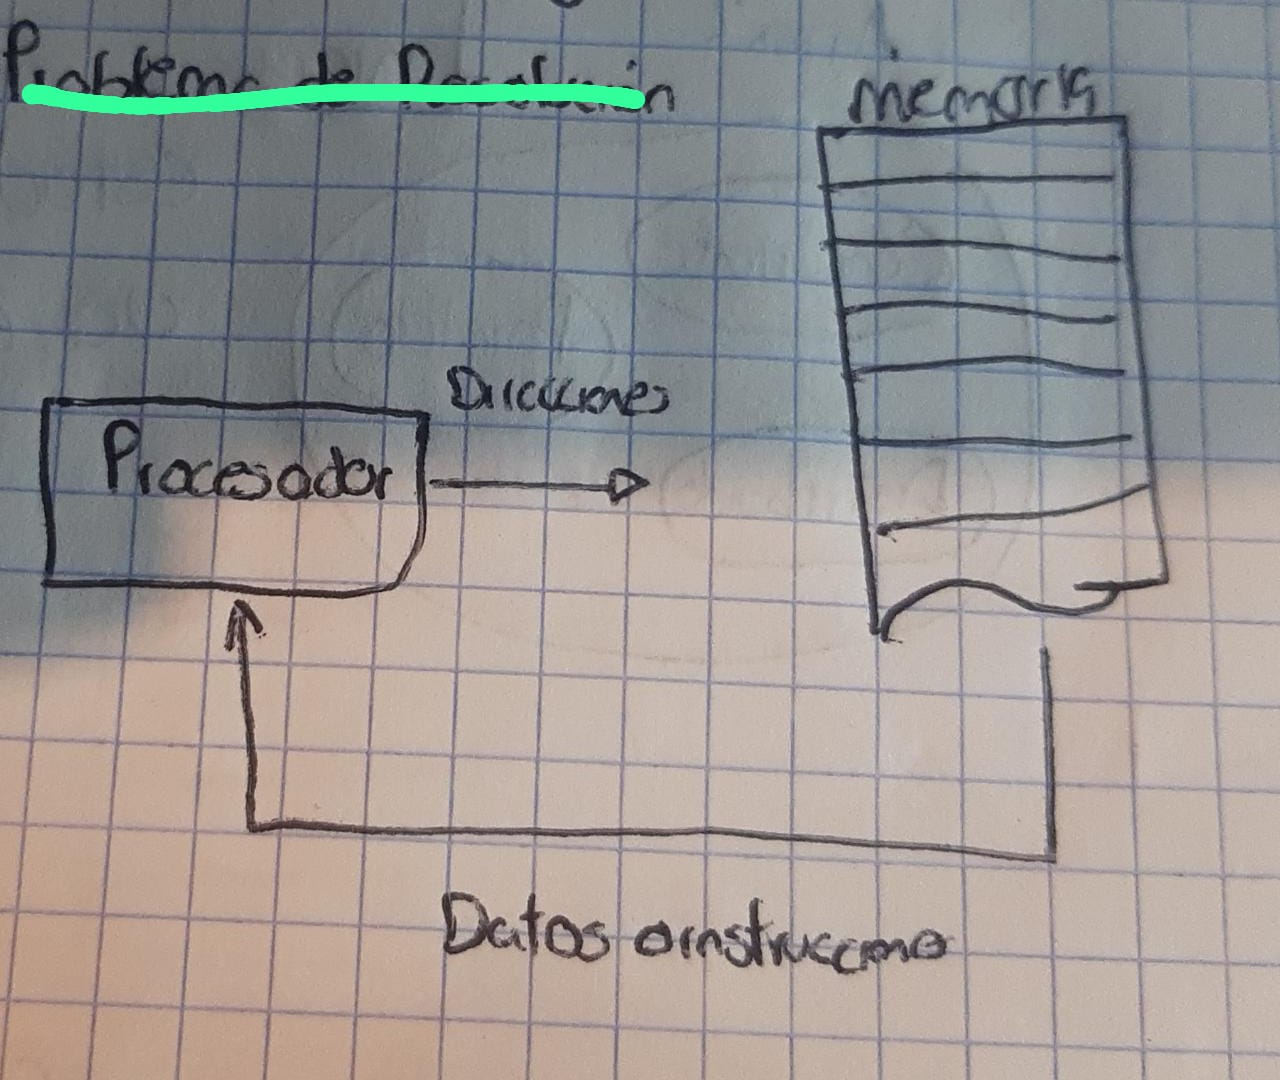
\includegraphics[scale = 0.25]{images/esquema1.jpeg} \\

{\color{blue} \subsection*{\textbf{Instrucciones y datos en memoria codificados.}}}
En la ejecución de un programa se siguen varios pasos, como lo son:\\
\begin{enumerate}
    \item FETCH: Obtener o buscar las instruciones.
    \item DECODE: De que trata (decodificación).
    \item EXECUTE: Ejecución de la instrucción.
    \item WRITE: Se escribe en el caso de sincronia para el proceso.
\end{enumerate}

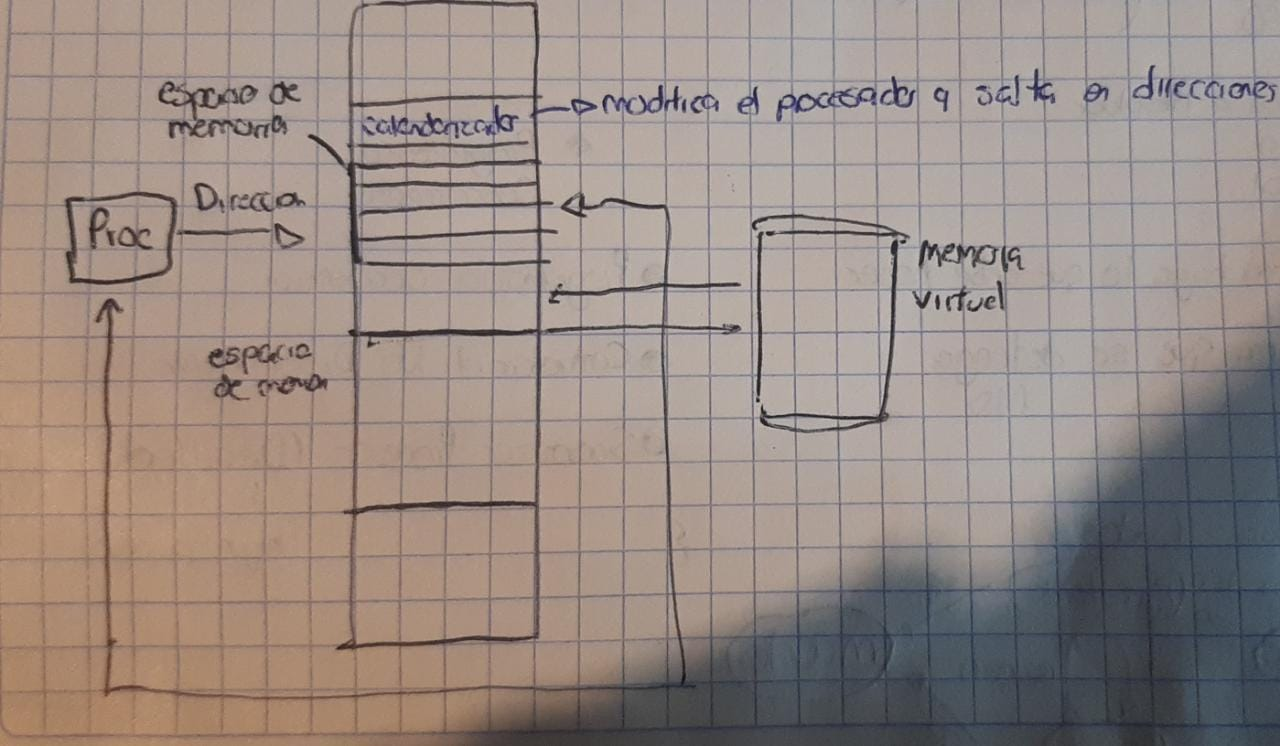
\includegraphics[scale = 0.30]{images/esquema2.jpeg} \\

{\color{blue} \subsection*{\textbf{Memoria compartida.}}}
Se encarga de comunicar procesos mediante la variable global (\textbf{Variable Compartida}).
Todos los procesadores acceden a una memoria global \\

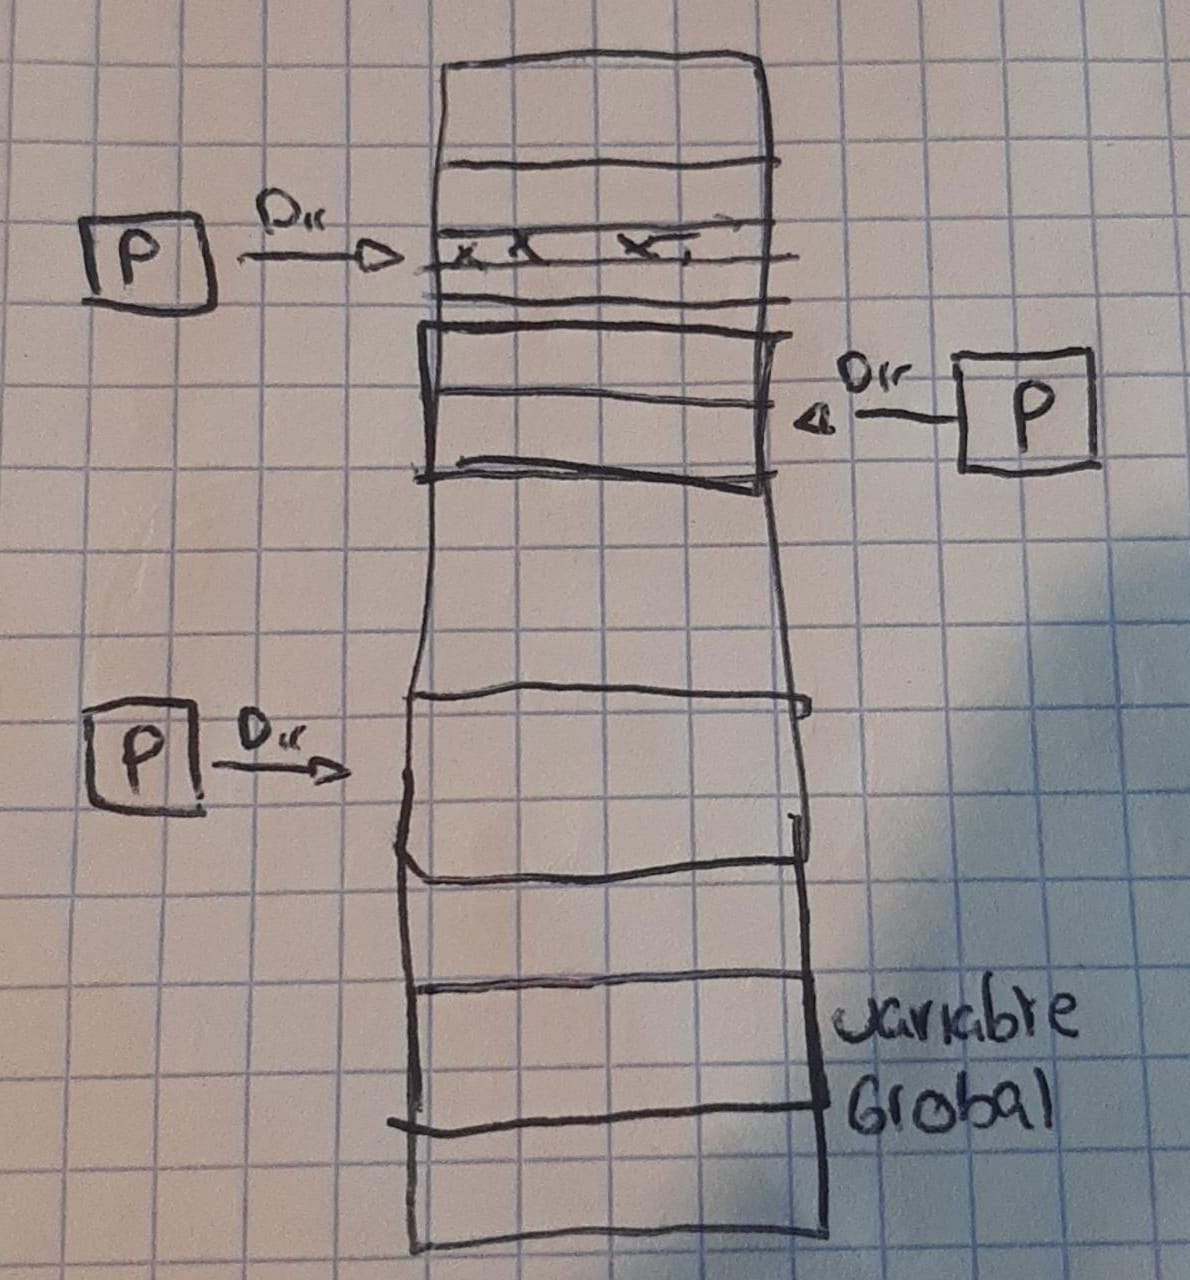
\includegraphics[scale = 0.30]{images/esquema3.jpeg} \\

{\color{blue} \subsection*{\textbf{Memoria Distribuida.}}}
Cada procesador tiene su memoria local intercambiando datos mediante una red de comunicación \textbf{(E/S)}\\

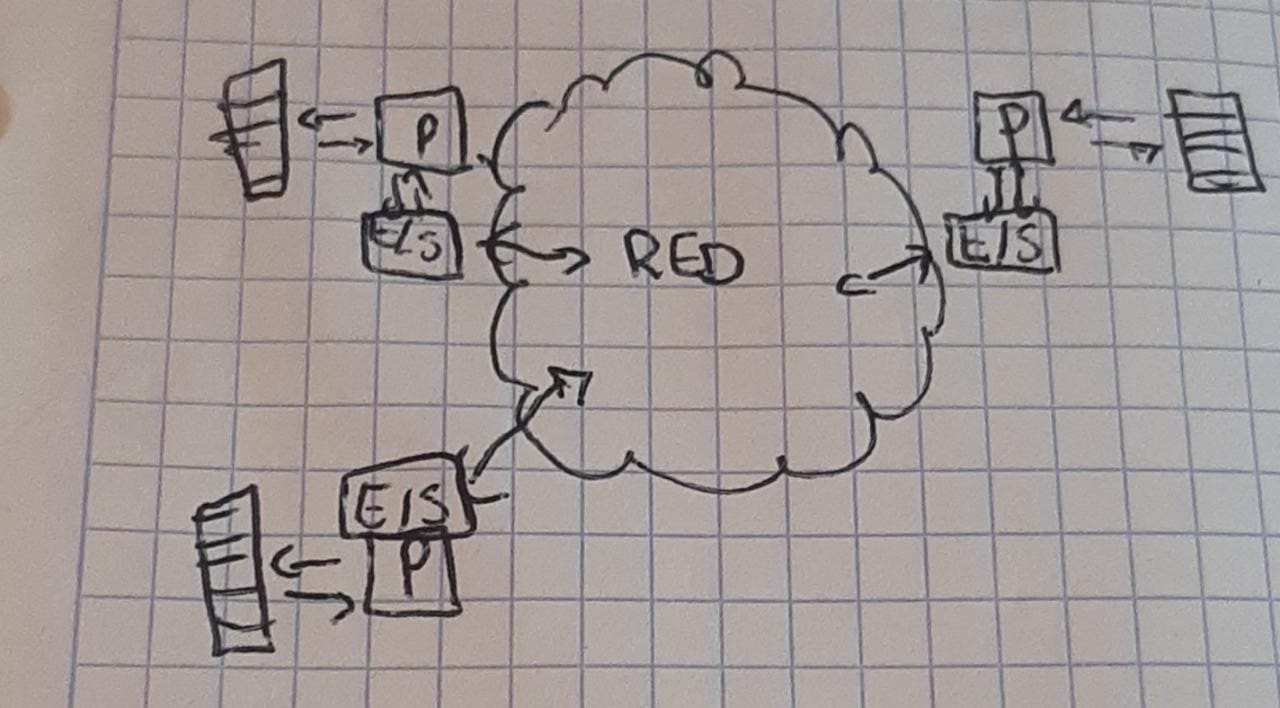
\includegraphics[scale = 0.35]{images/esquema4.jpeg} \\

{\color{blue} \subsection*{\textbf{LENGUAJE DE PROGRAMACIÓN.}}}
\vspace{1em}

\begin{enumerate}
    \item \textbf{Expresar Concurrencia:} OCAN: PAR, ---- parbegin y parend. {\color{red}*preguntar el leguaje occan y otro}
    \item \textbf{Expresar Secuencialidad:} ($P_{1}; P_{2}$;) instrución secuencial, OCCAN: (SEQ)
    \item \textbf{Expresar Comunicación:} Depende de la organización de la memoria.
    \begin{enumerate}
        \item \textbf{Compartida:} Variable Compartida.
        \item \textbf{Distribuida:} Llamada a procedimientos Remotos y paso de mensajes \color{red} send(), recerver()
    \end{enumerate}
    \item \textbf{Control del NO-Determinismo:} No todos, esto significa que antes de ejecutarlo no sabremos que pasará. Conjunto de 
    estados no se sigue rigurosamente.\\
    Instrución alternativa de Dijktra: Instrucción concurrentemente o al mismo tiempo y sin parar.
\end{enumerate}

(threads en java nos dan la concurrencia)

{\color{blue} \subsection*{\textbf{Inclusión de concurrencia en Lenguajes de Programación.}}}
\begin{enumerate}
    \item Diseño del Lenguaje (Occan).
    \item Modificando el lenguaje.(extención en el compilador).
    \item Utilizando bibliotecas (libres).
\end{enumerate}
\vspace{2em}

{\color{blue} \subsubsection*{\textbf{Problema a Resolver.}}}

Programa $=$ Algoritmo $+$ Datos.

({\color{red} \textbf{Capacidad de dividir el algoritmo ó datos para programar en paralelo.}})\\

{\color{red} \textbf{Programa Concurrente:}} Componentes de procesamiento $+$ Componentes de comunicación.\\

{\color{blue} \subsection*{\textbf{Conceptos y Terminología.}}}
\vspace{1em}

{\color{red} \textbf{Proceso.}} Es el cambio en el \textbf{estado} de la memoria por acción del procesador. (valor instantaneo de las variables de un sistema.)\\

{\color{red} \textbf{Programa.}} Es la especificación de uno o varios procesos. (ya sea \textbf{secuencial} o \textbf{concurrente}.)
\vspace{2em}\\

\begin{enumerate} 
    \item {\color{red} \textbf{Programación Secuencial.}} Especificación de un proceso.
    \item {\color{red} \textbf{Programación Concurrente.}} Especificación de varios procesos.\\
    Conjunto de de procesos secuenciales que se ejecutan simultaneamente, comunican entre si por un objetivo en común.
    \begin{enumerate}
        \item \textbf{Programa Multithread.}
        \item \textbf{Programa Paralelo.}
        \begin{enumerate}
            \item Memoria compartida: comunicación por memoria.
            \item Memoria Distribuida: Reedes Compartidas.
        \end{enumerate}
        \item \textbf{Programas Distribuidos.}
    \end{enumerate}
\end{enumerate}

\begin{tabular}{| c | c |}
    \hline
    \textbf{Cnceptos de SW} & \textbf{Cnceptos de HW} \\ \hline
    Proceso & Procesador \\
    Comunicación(variable compartida (global.\\
    Paso de mensajes y llamadas a procedimientos remotos)) & Memoria (Distrib y Compartida).
\end{tabular}\\

*(procesador accede a la memoria en nano segundos)\\
* Los factores son: plataforma de HW, lenguajes de programación y el problema a resolver.
\vspace{2em}

{\color{blue} \subsubsection*{\textbf{Coordinación:}}}
Establecer puntos de acciones en tiempo y espacio.\\
Organizar las tareas de tal forma que esten en tiempo y espacio y no tarden en comunicarse. (termina en tiempo) 
\vspace{1em}

{\color{blue} \subsubsection*{\textbf{Comunicación.}}}
Intercambio de mensajes.
\vspace{1em}

{\color{blue} \subsubsection*{\textbf{Sincronización.}}}
Protocolo para intercambio de forma ordenada.\\
Acciones para realizar la comunicación de forma exitosa. Para ello necesitamos la sincronización de las formas de comunicación.
\vspace{1em}

{\color{blue} \subsubsection*{\textbf{Granularidad..}}}
Que tanto es o se puede dividir algo. se usa la formula:  $G=\frac{tiempoProcesamiento}{tiempoComunicacion}$ \\
\begin{enumerate}
    \item \textbf{Gruesa:} (acceso controlado a BD, uno y uno). $G=\frac{mas}{menos}$
    \item \textbf{Media:} $G=\frac{normal}{normal}$
    \item \textbf{Fina:} (comunicación entre procesadores). $G=\frac{menos}{mas}$
\end{enumerate}
\vspace{1em}

{\color{blue} \subsection*{\textbf{TEMA 2: PROCESO SECUENCIAL.}}}
\vspace{1em}

{\color{blue} \subsubsection*{\textbf{Proceso Secuencial.}}}

Es el cambio de estado en la memoria por acción del procesador. Una instrucción a la vez ya que solo tiene un procesador.
\\

{\color{blue} \subsubsection*{\textbf{Arquitectura Von Neumman.}}}
\vspace{1em}
\begin{enumerate}
    \item Instrucciones y datos.
    \begin{enumerate}
        \item Almacenados en memoria.
        \item Codificados (binary).
    \end{enumerate}
    \item Thread (hilo de control): Como una hebra de control y cada instrucción es un caso al que se le agrega.
\end{enumerate}

Programa con un solo thread es proceso secuencial.\\

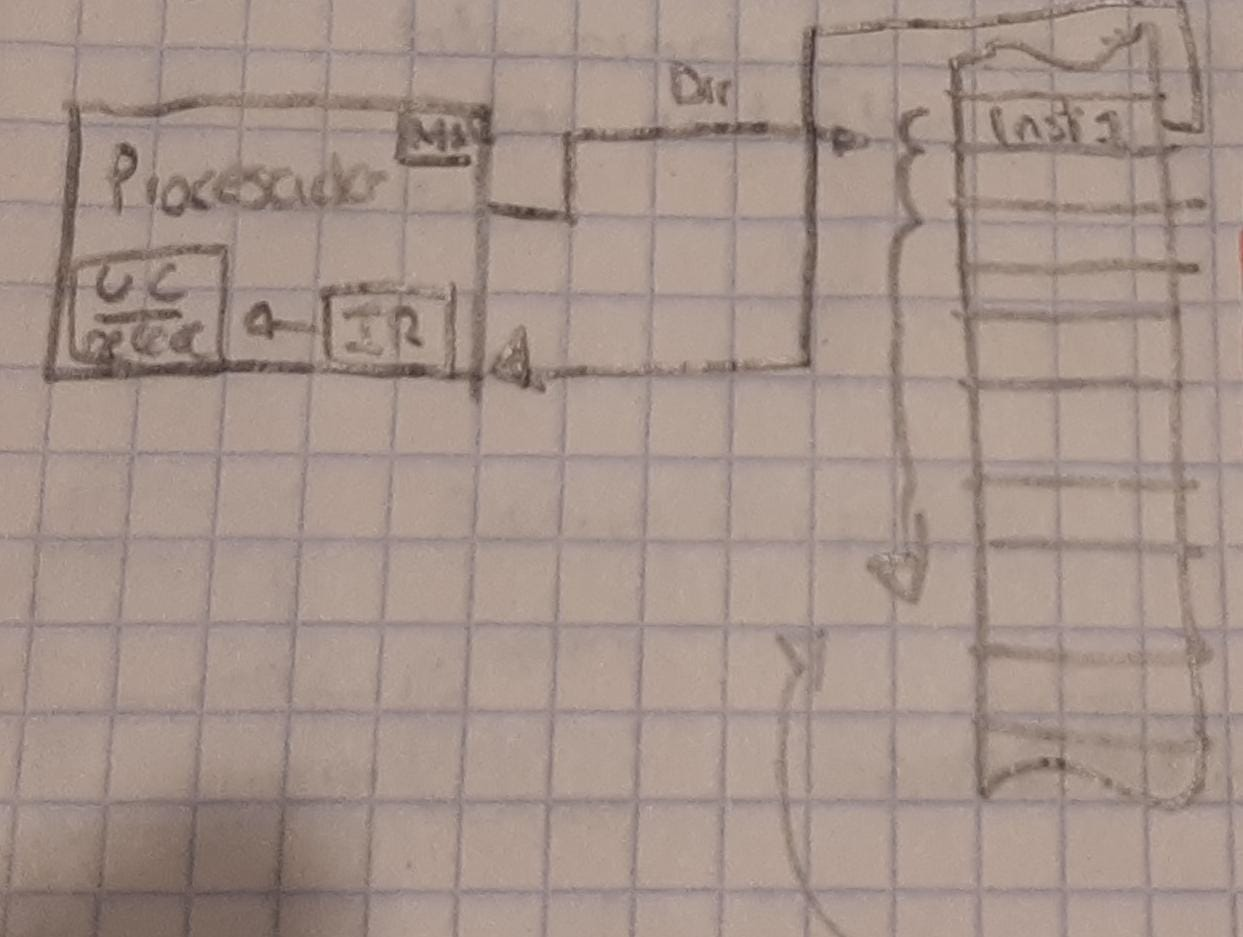
\includegraphics[scale = 0.25]{images/esquema5.jpeg} \\

Todo lo siguiente se ejecuta en un solo hilo o thread:
\begin{enumerate}
    \item FETCH(buscar)
    \item DECODE(comunicar)
    \item EXECUTE(ejecutar):
    \begin{enumerate}
        \item SW a HW.
        \item De instrucción lógica a señal fisica.
    \end{enumerate}
    \item WRITE(resultado): Determina la dirección de la siguiente instrucción.
\end{enumerate}

{\color{blue} \subsubsection*{\textbf{Lógica de transferencia de registros.}}}
\vspace{1em}

MAR $\leftarrow$ PC (microoperación)\\

\includegraphics*[scale = 0.25]{images/esquema6.jpeg} PC $\rightarrow$ Entre direcciones\\

\begin{enumerate}
    \item \textbf{FETCH}
    \begin{enumerate}
        \item $t_0 : MAR \leftarrow PC$
        \item $t_1 : MBR \leftarrow M$, $PC \leftarrow PC+1$
        \item $t_2 : IR \leftarrow MBR$
        \item NOP $q_0t_3 : T \leftarrow \emptyset$
        \item MOVR $q_1t_3 : A \leftarrow R, T \leftarrow \emptyset$
        \item LDI(Data8) $q_2t_3 : MAR \leftarrow PC$
        \item $q_0t_4 : MBR \leftarrow M$, $PC \leftarrow PC+1$
    \end{enumerate}
\end{enumerate}
\vspace{1em}

{\color{blue} \subsubsection*{\textbf{Instrucciones:}}}
Autocontención.
\\
{\color{blue} \subsubsection*{\textbf{CARACTERISTICAS DEL PROCESO SECUENCIAL:}}}
\begin{enumerate}
    \item \textbf{Que el programa haga lo que debe hacer.}
    \item \textbf{El proceso termine.}
\end{enumerate}


{\color{blue} \subsection*{\textbf{TEMA 3: PROCESOS CONCURRENTES.}}}
\vspace{1em}

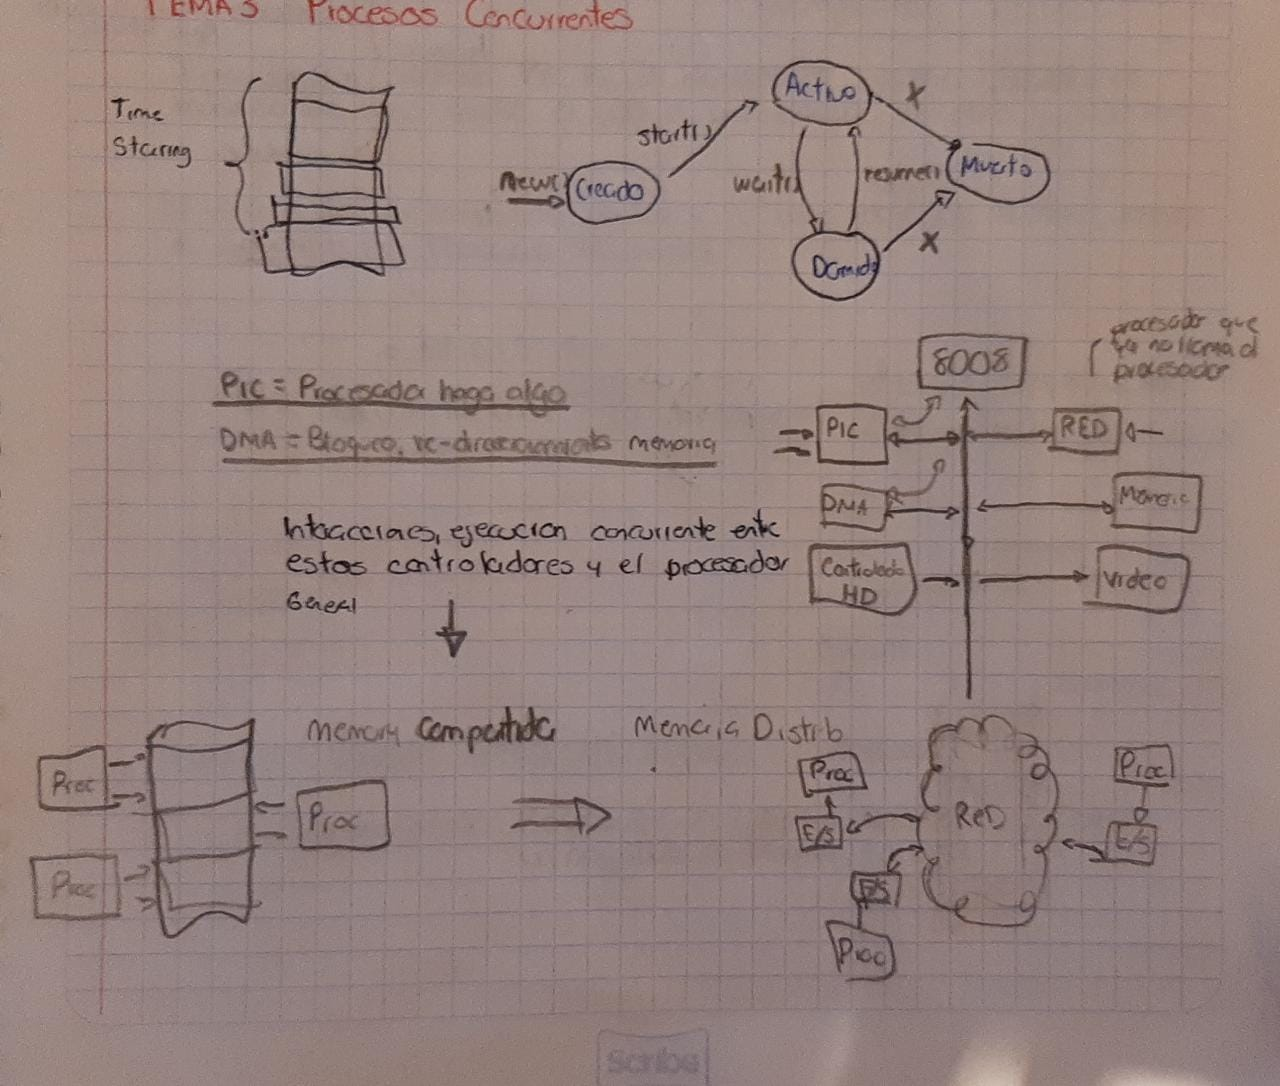
\includegraphics[scale = 0.34]{images/esquema7.jpeg} \\

{\color{blue} \subsubsection*{\textbf{Lenguaje Programación.}}}
\vspace{1em}
Expresión de comunicación (organiza la memoria.)
\begin{enumerate}
    \item Memoria Compartida: Usa Variable compartida.
\end{enumerate}

{\color{blue} \subsection*{\textbf{Co-operating Sequenlid E.W.D.}}}
\vspace{1em}
\begin{enumerate}
    \item {\color{red}\textbf{Contexto:}} Memoria compartida. \textbf{Procesos concurrentes comunicandose por variables compartidas}
    \item {\color{red}\textbf{Problema:}} Variables compartidas tienen un valor $\rightarrow$ \textbf{Integridad con exclusión mutua} 
    \item {\color{red}\textbf{Solución:}} Semaforo $\rightarrow$ \textbf{Exclusión mutua} $\rightarrow$ \textbf{Sección critica}\\
    Se mezclan los procesos $P_a$, $P_b$ al momento de ejecutar \textbf{FDXR} al momento que no escribe el valor de una variable, el otro igual lo hace.\\

\end{enumerate}

* El valor de la variable compartida cambia y no tiene integridad y hace perdida de actualizaciones. ({\textbf{Procesador secuencial}}).\\

\textbf{Sección Critica:} Parte del codigo que modifica la variable compartida.

\begin{verbatim}
    1.                       int a = 1;
    2.  PA for(for 20 veces):         PB for(for 20 veces):
    3.      a++                              a++
    4. 
    5.  //El que lee, ¿qué lee?
    6.  //El que escribe, ¿qué escribe?
    7. // esto cuando 
\end{verbatim}

En un crucero, en donde se cruzan los autos por decir, los autos son los procesos y la intercepción es la \textbf{Sección critica.}\\

\textbf{Semaforo:} Variable entera NO-Negativa.
\begin{enumerate}
    \item \textbf{P:} Disminuye el valory en caso bloquea.
    \item \textbf{V:} Aumenta el valor.
\end{enumerate}

\textbf{P:(Operación bloqueante)}: Proceso que lo invoque y si da negativo, este se bloquea y no sigue.

{\color{blue} \subsection*{Sincronización en Variable Compartida.}}

No anidar seccion critica.\\

\begin{enumerate}
    \item Semaforo $\rightarrow$ Bloqueante.
    \item Algoritmo de Decker $\rightarrow$ \textbf{Espera activa}.
    \item Region Critica
    \item Monitor.
\end{enumerate}

\textbf{ESPERA ACTIVA:} En el caso del algoritmo de becker el $c_2$ si no cambia y sigue esperando, regresa y sigue sin cambiar, es como si diera vueltas
en un carrusel, por tanto es dar vueltas y esperar y esperar y esperar.\\
Consume tiempo del procesador (\textbf{Polling}).\\

{\color{blue} \subsubsection*{Productor-Consumidor.}}
\vspace{1em}

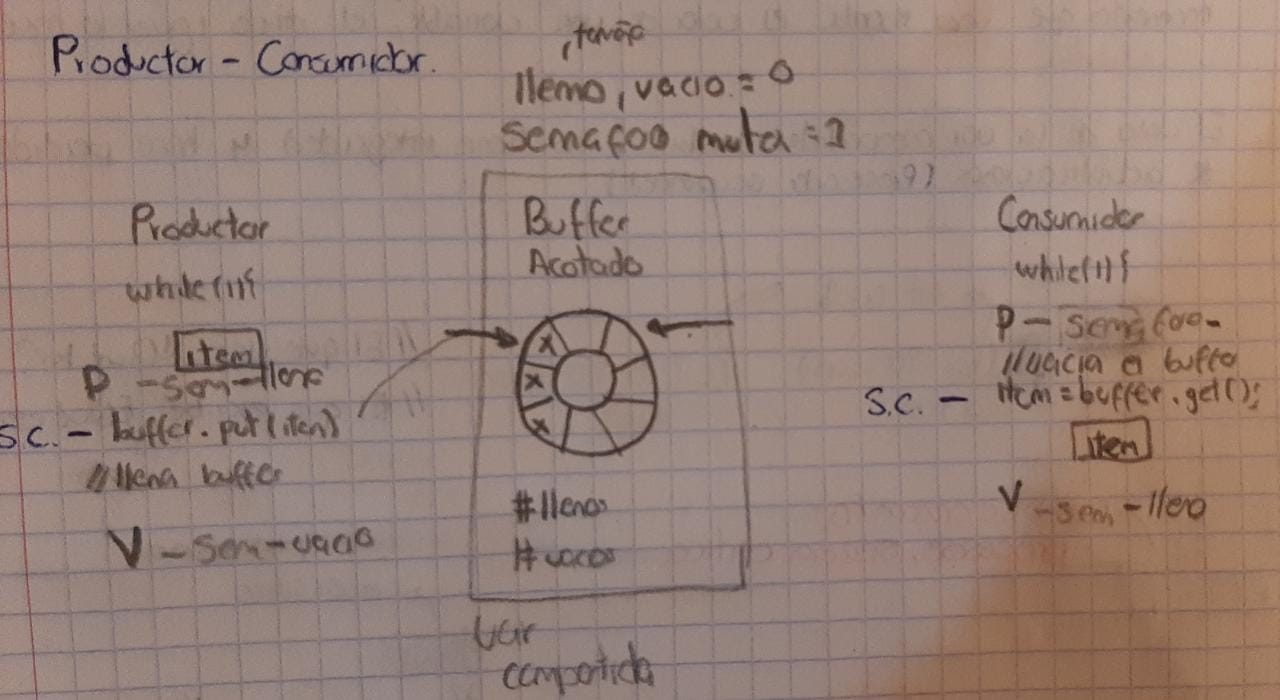
\includegraphics[scale = 0.40]{images/esquema8.jpeg} \\













\end{document}